\documentclass[aspectratio=169]{beamer}

\mode<presentation>
\usetheme{Boadilla}
\definecolor{redback}{RGB}{140,0,0}
\definecolor{blue}{RGB}{30,90,205}
\definecolor{red}{RGB}{213,94,0}
\definecolor{green}{RGB}{0,128,0}
\setbeamercolor{title}{fg=redback}
\setbeamercolor{frametitle}{fg=redback}
\setbeamercolor{block title}{bg=redback, fg=white}
\setbeamercolor{block body}{bg=white}
\setbeamercolor{structure}{fg=redback}
\setbeamercolor{item projected}{fg=white}
\setbeamercolor{item}{fg=redback}
\setbeamercolor{subitem}{fg=redback}
\setbeamercolor{section in toc}{fg=redback}
\setbeamercolor{description item}{fg=redback}
\setbeamercolor{caption name}{fg=redback}
\setbeamercolor{button}{bg=redback, fg=white}
\setbeamercolor{caption name}{fg=redback}
\usepackage{graphics}
\usepackage{tikz}
\usepackage{amsmath}
\usepackage{bbm}
\usetikzlibrary{decorations.pathreplacing}
\usepackage{geometry}
\usepackage{booktabs}
\usepackage{multirow, makecell}
\usepackage{float}
\usepackage{fancyvrb}
\usepackage{kotex}
\usepackage{caption}
\usepackage{subcaption}
\usepackage{adjustbox}
\usepackage{hyperref}
\usepackage{threeparttable}
\usepackage[scaled=0.92]{helvet}
\usepackage[default]{lato} %If I want a twist
\newenvironment{wideitemize}{\itemize\addtolength{\itemsep}{10pt}}{\enditemize}
\newenvironment{wideenumerate}{\enumerate\addtolength{\itemsep}{10pt}}{\endenumerate}
\newenvironment{widedescription}{\description\addtolength{\itemsep}{10pt}}{\enddescription}
\hypersetup{
colorlinks=true,
linkcolor=redback,
filecolor=green, 
urlcolor=blue,
}
\beamertemplatenavigationsymbolsempty
\setbeamercolor{author in head/foot}{bg=white, fg=redback}
\setbeamercolor{title in head/foot}{bg=white, fg=redback}
\setbeamercolor{date in head/foot}{bg=white, fg=redback}
\setbeamercolor{section in head/foot}{bg=white, fg=redback}
\setbeamercolor{page number in head/foot}{bg=white, fg=redback}
\setbeamercolor{headline}{bg=redback}
\setbeamertemplate{footline}{
    \leavevmode%
    \hbox{%
        \begin{beamercolorbox}[wd=.333333\paperwidth,ht=2.25ex,dp=1ex,center]{date in head/foot}%
            \usebeamerfont{date in head/foot}\insertshortdate
        \end{beamercolorbox}%
        \begin{beamercolorbox}[wd=.444444\paperwidth,ht=2.25ex,dp=1ex,center]{title in head/foot}%
            \usebeamerfont{title in head/foot}\insertshorttitle
        \end{beamercolorbox}%
        \begin{beamercolorbox}[wd=.222222\paperwidth,ht=2.25ex,dp=1ex,center]{page number in head/foot}%
            \usebeamerfont{page number in head/foot} \insertframenumber{} / \inserttotalframenumber
        \end{beamercolorbox}}%
        \vskip0pt%
    }

\setbeamertemplate{section in toc}[sections numbered]
\setbeamertemplate{subsection in toc}{\leavevmode\leftskip=3em\rlap{\hskip-1.75em\inserttocsectionnumber.\inserttocsubsectionnumber}\inserttocsubsection\par}
\setbeamerfont{subsection in toc}{size=\footnotesize}

\newenvironment{transitionframe}{\setbeamercolor{background canvas}{bg=redback}\setbeamertemplate{footline}{} \begin{frame}}{\end{frame}}
\newcommand{\ROM}[1]
    {\MakeUppercase{\romannumeral #1}}

\makeatletter
\let\@@magyar@captionfix\relax
\makeatother


\title[Recitation 3 (Intro to Econometrics \ROM{2})]{Recitation 3: Various tests in IV-GMM framework} % Change this regularly
\author[]{Seung-hun Lee }
\institute[]{Columbia University \\ Introduction to Econometrics \ROM{2} Recitation}

\date[February 7th, 2022]{February 7th, 2022}

\begin{document}
\begin{frame}
\titlepage
\end{frame}


%%% Color slides for section headers: Use for colloquium version (The ones bewteen \iffals and \fi)

\begin{transitionframe}
  \begin{center}
         { \Huge \textcolor{white}{Primer on Wald vs LM vs LR tests}}
       \end{center}
\end{transitionframe}



\begin{frame}
\frametitle{Engle (1984): Wald uses unconstrained estimator and its distance}
\begin{itemize}
\item Suppose we have the data $y$, parameter of interest $\beta$ and the log likelihood function $L(y,\beta)$. The hypothesis we want to check is
\[
H_0:\beta=\beta_0 \ \text{vs} \ H_1: \beta\neq\beta_0
\]
\item Wald: This is a test based on unconstrained regression in the sense that it tests the composite alternative hypothesis against the null. The idea is to accept the null when the estimated value of $\beta$ is reasonably close to $\beta_0$. The typical test statistics is
\[
t_{W} = (\hat{\beta}-\beta_0)'(var(\hat{\beta}))^{-1}(\hat{\beta}-\beta_0) \sim \chi^2_{\dim{(\beta)}}
\]

\end{itemize}
\end{frame}


\begin{frame}
\frametitle{Engle (1984): LM uses constrained regressions}
\begin{itemize}
\item LM: This is based on the constrained minimization problem of the likelihood function. We impose the null hypothesis with the following constrained optimization problem
\[
L(y,\beta)-\lambda'[\beta-\beta_0]
\]
with the first order conditions
\begin{itemize}
\item With respect to $\beta$:  $\frac{\partial L}{\partial \beta} = \lambda$
\item With respect to $\lambda$: $\beta=\beta_0$
\end{itemize}
By complementary slackness conditions, we would have $\lambda\geq0$ and $\lambda=0$ if the constraint is not binding. If the shadow price is high (high $\lambda=s(y,\beta_0)$), then we would reject the constraint. Typically, the test statistics used has this form:
\[
t_{LM} = s(y,\beta_0)'(var(s))^{-1}s(y,\beta_0) \sim \chi^2_{\dim(\beta)}
\]
\end{itemize}
\end{frame}


\begin{frame}
\frametitle{Engle (1984): Use both restricted and unrestricted regressions}
\begin{itemize}
\item LR: This is based on the difference between the maximum of the likelihood under the null vs under the alternative. Typically, the test statistics have the following form
\[
t_{LR} = -2[L(y,\beta_0)-L(y,\hat{\beta})]\sim \chi^2_{\dim(\beta)}
\] 
\item In short, 
\begin{figure}[H]
\begin{center}
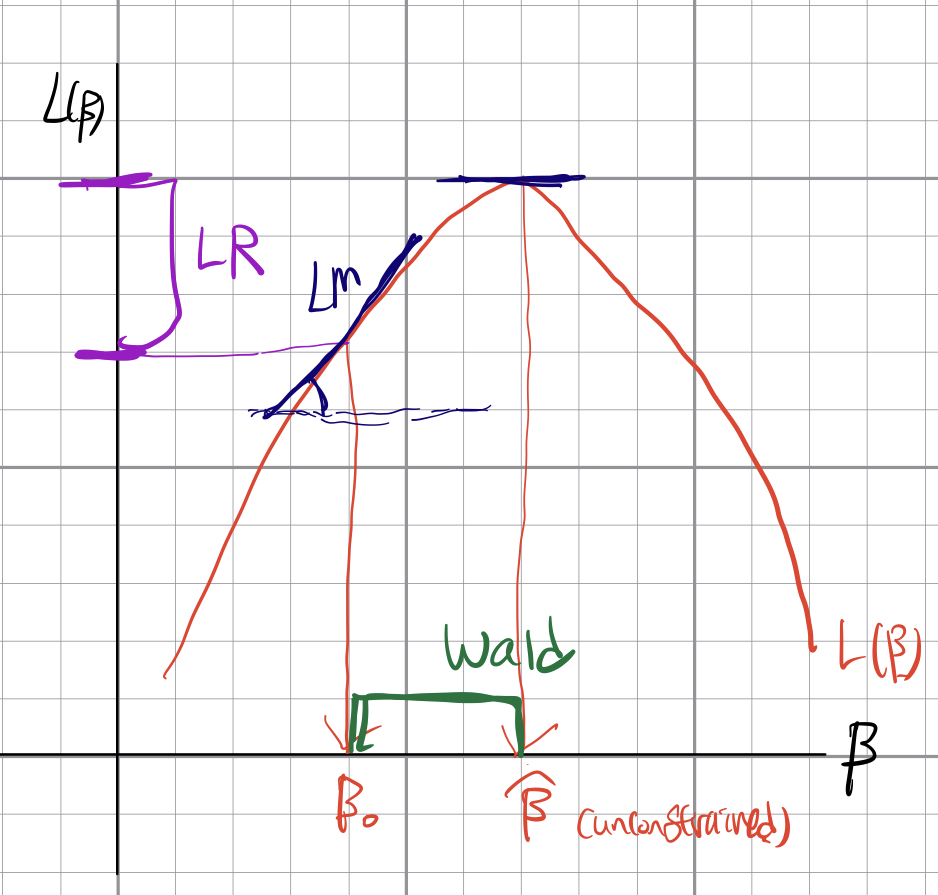
\includegraphics[width=0.3\textwidth, keepaspectratio]{3test.jpeg}
\caption{Wald vs LM vs LR}
\end{center}
\end{figure}
\end{itemize}
\end{frame}


\begin{transitionframe}
  \begin{center}
         { \Huge \textcolor{white}{Tests of exongeneity and endogeneity}}
       \end{center}
\end{transitionframe}

\begin{frame}
\frametitle{Hansen's test: Are the (overidentified) instruments really exogenous?}
\begin{itemize}
\item Setup: $k$ covariates $x_i$ and $l$-vector instrument $z_i$ ($l>k$)
\item Hansen's J-test: $H_0: E[g(w_i,\beta)]=0 \ \text{vs. } H_1: E[g(w_i,\beta)]\neq0$ where $g(w_i,\beta)=z_ie_i$
\begin{itemize}
\item Make use of a GMM criterion: $J(\beta)=n\bar{g}(\beta)'\widehat{\Omega}^{-1}\bar{g}(\beta)$. 
\item Asymptotics: 
\[
J(\beta)= \underbrace{\left(\sqrt{n}\bar{g}(\beta) \right)'}_{\xrightarrow{d}N(0,\Omega)} \widehat{\Omega}^{-1}\underbrace{\left(\sqrt{n}\bar{g}(\beta) \right)}_{\xrightarrow{d}N(0,\Omega)}\xrightarrow{d} \chi^2_l
\]
\item However, we need an estimate of $e_i$ using $\hat{\beta}_{GMM}$.
\item We really do this with $J(\hat{\beta}_{GMM})\sim  \chi_{l-k}^2$. (We estimate $k$ parameters)
\item For significance level $\alpha$, compare $J(\hat{\beta}_{GMM}$ with $\chi_{l-k, \alpha}^2$ where $\Pr(\chi^2\geq\chi_{l-k, \alpha}^2) = \alpha$
\end{itemize}
\item The test introduced here also tests for other issues with the specification, so it is possible to reject this test for reasons other than instrument endogeneity
\item This is robust to heteroskedasticity (We have not set any restrictions on $\Omega = E[z_iz_i'e_i^2]$)
\end{itemize}
\end{frame}

\begin{frame}
\frametitle{Sargan's test: Hansen's test with homoskedasticity}
\begin{itemize}
\item Assume
\[
y_i = x_i'\beta+e_i \ (\dim(x_i)=k<\dim(z_i)=l) 
\]
\item Construct a linear projection equation by projecting $e_i$ onto $z_i$, obtaining
\[
e_i=z_i'\delta+\epsilon_i \to\delta=E(z_iz_i')^{-1}E(z_ie_i)
\]
\item So we need to test $H_0: \delta=0$ vs. $H_1: \delta\neq0$
\begin{itemize}
\item  \textbf{Obtain $\hat{e}_i$}: This can be done using 2SLS estimates of $\beta$
\item \textbf{Obtain $\hat{\delta}$}: Replace $e$ with $\hat{e}$ to get $\hat{\delta} = (Z'Z)^{-1}Z'\hat{e}$
\textbf{Sargan Test}: Assuming homoskedasticity, we use 
\[
S=\hat{\delta}'(var(\hat{\delta}))^{-1}\hat{\delta}=\frac{\hat{e}'Z(Z'Z)^{-1}Z'\hat{e}}{\hat{\sigma}^2}\xrightarrow{d}\chi_{l-k}^2 \  \ \ (\hat{\sigma}^2=\frac{1}{n}\hat{e}'\hat{e})
\]
\end{itemize}
\item Same caution as before applies!
\end{itemize}
\end{frame}


\begin{frame}
\frametitle{Subset exogeneity test: Some are certain, but others are not}
\begin{itemize}
\item Partition $z_i$ into two sets - $z_{ai}\in\mathbb{R}^{l_a}$ and $z_{bi}\in\mathbb{R}^{l_b}$. 
\item We are uncertain about $z_{bi}$ and want to test 
\[
H_0: E(z_{bi}e_i)=0, \ \text{vs. }H_1:E(z_{bi}e_i)\neq0
\]
\item Distance-test: Are GMM criterion values similar?
\begin{itemize}
\item  Estimate the model by the efficient GMM with only the $z_{ai}$ set of instruments and obtain the GMM criterion $J_a$
\item  Estimate the model with the full set of instruments and obtain a separate GMM criterion, denoted as $J_{a,b}$
\item Then, create a test statistic
\[
C=J_{a,b}-J_a\xrightarrow{d}\chi^2_{l-l_a=l_b}
\]
\item Find critical value $\chi_{l_b,\alpha}^2$ for a significance level $\alpha$ and reject the null hypothesis if $C>\chi_{l_b,\alpha}^2$
\end{itemize}
\end{itemize}
\end{frame}

\begin{frame}
\frametitle{Other ways to do subset exogeneity test}
\begin{itemize}
\item Amemiya-Lee-Newey: Use an auxiliary regression
\begin{itemize}
\item Project $e_i$ onto the ones we are certain about ($z_a$) and the ones we are not ($z_b$)
\[
e_i = z_{ai}'\delta_a+z_{bi}'\delta_b+u_i
\]
\item Test for the exogeneity of $z_b$ instruments by checking $\delta_b=0$
\item In practice: Obtain residuals $\hat{e}$ and run an auxiliary regression of this into the two sets of instruments and obtain estimates for $\delta_b$
\item  The test statistics used and its distribution under the null is
\[
\hat{\delta}_b'(\text{var}(\hat{\delta}_b))^{-1}\hat{\delta}_b \sim \chi_{l_b}^2
\] 
\end{itemize}
\end{itemize}
\end{frame}

\begin{frame}
\frametitle{Hausman test can be used here too!}
\begin{itemize}
\item Using Hausman principle
\begin{itemize}
\item  Obtain two estimates of $\beta$ - one using only the sure IVs and the other using all sets of IVs
\item Then, the idea is to check whether the two estimates are close to each other. 
\end{itemize}
\item To use this
\begin{itemize}
\item Make sure $z_a$ is always exogenous
\item We need to make sure that $z_a$ is a consistent yardstick to compare the full set of instruments against
\end{itemize}
\end{itemize}
\end{frame}

\begin{frame}
\frametitle{Hausman principles: Key is getting the right two estimators}
\begin{itemize}
\item Hausmann Test can be utilized as a general test of specification. 
\item It is aimed at testing the consistency of an estimator that we are uncertain about relative to an estimator that is surely consistent. 
\item The general trick is that you need two types of estimators. 
\begin{itemize}
\item $\hat{\theta}_1$: Consistent and efficient under $H_0$, inconsistent under $H_1$
\item $\hat{\theta}_2$: Consistent in either $H_0$ or $H_1$. Inefficient under $H_0$. 
\end{itemize}
\item Then the difference between the two estimators have the following asymptotic distribution
\[
\sqrt{n}(\hat{\theta}_1-\hat{\theta}_2) \sim N(0, \text{var}(\hat{\theta}_2-\hat{\theta}_1))
\]
\item The test statistic that is used is
\[
H=(\hat{\theta}_1-\hat{\theta}_2)'(\text{var}(\hat{\theta}_2-\hat{\theta}_1))^{-1}(\hat{\theta}_1-\hat{\theta}_2)
\] 
\end{itemize}
\end{frame}

\begin{frame}
\frametitle{Endogeneity/Exogeneity of regressors $x_i$}
\begin{itemize}
\item Assume that homoskedasticity is satisfied and the data generating process is
\[
y_i = x_{1i}'\beta_1 + x_{2i}'\beta_2+e_i
\]
\item We test $H_0: E(x_{2i}e_i)=0$ against $H_1:E(x_{2i}e_i)\neq0$
\item Consider these properties of 2SLS and OLS estimators
\begin{itemize}
\item $\hat{\beta}_{OLS}$: Consistent and minimal variance under $H_0$, inconsistent under $H_1$
\item $\hat{\beta}_{2SLS}$:  Consistent in either $H_0$ or $H_1$. Inefficient under $H_0$. 
\end{itemize}
\item Under $H_0$, $\sqrt{n}(\hat{\beta}_{2SLS}-\hat{\beta}_{OLS})$ converges in distribution to $N(0, var(\hat{\beta}_{2SLS}-\hat{\beta}_{OLS}))$
\item Hausman: $var(\hat{\beta}_{2SLS}-\hat{\beta}_{OLS})=var(\hat{\beta}_{2SLS})-var(\hat{\beta}_{OLS})$ holds in homoskedasticity
\item Thus the Hausman test statistic
\[
(\hat{\beta}_{2SLS}-\hat{\beta}_{OLS})'(var(\hat{\beta}_{2SLS})-var(\hat{\beta}_{OLS}))^{-1}(\hat{\beta}_{2SLS}-\hat{\beta}_{OLS})\xrightarrow{d}\chi_{k_2}^2
\]\
\end{itemize}
\end{frame}


\begin{frame}
\frametitle{Using Control function is also possible}
\begin{itemize}
\item  Assume the following setup
\[
\begin{aligned}
y_i &= x_{2i}'\beta_2+e_i& \ \ (E[x_{2i}e_i]\neq0) \\
x_{2i}&=z_i'\pi_2 + v_{2i}& \ \ (E[z_ie_i]=0, E[z_iv_{2i}]=0)\\
e_i &=v_{2i}'\rho + w_i&\\
y_i &= x_{2i}'\beta_2+v_{2i}\rho + w_i
\end{aligned}
\]
\item Replace this with $\hat{v}_{2i}$ by running an OLS on the first stage regression and then write
\[
y_i = x_{2i}'\beta_2+\hat{v}_{2i}\rho + w_i
\]
\end{itemize}
\end{frame}

\begin{frame}
\frametitle{So what are we looking for?}
\begin{itemize}
\item What we need to do is to check whether $\hat{\rho}=0$ or not
\item Recall that
\[
E[x_{2i}e_i]=E[(z_i'\pi_2 + v_{2i})e_i]=E[v_{2i}e_i] \ (\because E[z_ie_i]=0)
\]
\item From the projection of $e_i$ onto $v_{2i}$
\[
\rho = E[v_{2i}v_{2i}']^{-1}E[v_{2i}e_i]\to\hat{\rho}=\frac{1}{n}\sum_{i=1}^n(v_{2i}v_{2i}') \frac{1}{n}\sum_{i=1}^n(v_{2i}e_i)
\]
\item If $x_2$ is exogenous, we would get $\rho=0$. So we would need to test whether $\hat{\rho}$ is close to zero or not. 
\end{itemize}
\end{frame}

\begin{frame}
\frametitle{Variable addition test and Hausman principle}
\begin{itemize}
\item Suppose that you found an instrumental variable (or variables) for your endogenous $X_2$, and that you went ahead with your 2SLS. 
\item Then you may suddenly wonder whether it was worth getting an IV to begin with. 
\item One way of testing for the endogeneity of your $X_2$ is to see if the 2SLS and the OLS estimates differ drastically.
\item The idea is that if there is not much endogeneity, the two estimates should be similar.
\item Note that
\[
\begin{aligned}
\hat{\beta}_{2SLS}&=(X'P_Z'X)^{-1}(X'P_Z'y)\\
\hat{\beta}_{OLS}&=(X'X)^{-1}(X'y)\\
\end{aligned}
\]
\end{itemize}
\end{frame}

\begin{frame}
\frametitle{So how do we make use of the differences?}
\begin{itemize}
\item The difference between the two is 
\[
\begin{aligned}
\hat{\beta}_{2SLS}-\hat{\beta}_{OLS}&=(X'P_Z'X)^{-1}(X'P_Z'y)-(X'X)^{-1}(X'y)\\
&=(X'P_Z'X)^{-1}[(X'P_Z'y)-(X'P_Z'X)(X'X)^{-1}(X'y)]\\
&=(X'P_Z'X)^{-1}X'P_Z'[y-X(X'X)^{-1}(X'y)]\\
&=(X'P_Z'X)^{-1}X'P_Z'[y-P_Xy]\\
&=(X'P_Z'X)^{-1}X'P_Z'[I-P_X]y\\
&=(X'P_Z'X)^{-1}X'P_Z'M_Xy\\
&=(\widehat{X}'X)^{-1}\widehat{X}'\widehat{e}\\
\end{aligned}
\]
\item The takeaway is that testing the endogeneity/exogeneity of $X$ with respect to $e$ is equivalent to testing for $X'P_Z'M_Xy=0$. 
\end{itemize}
\end{frame}

\begin{frame}
\frametitle{Building up the test statistics}
\begin{itemize}
\item In the original equation where we had $y=X\beta+e$, we add a regressor $\widehat{X}$. 
\item Effectively, we are working with an auxiliary regression in this form
\[
y=X\beta+\widehat{X}\gamma+\epsilon
\]
\item Note that the $\hat{\gamma}$ can be written as
\[
\begin{aligned}
\hat{\gamma}&=(\widehat{X}'M_X X)^{-1}(\widehat{X}'M_X y) \ (\because \text{Frisch-Waugh-Lovell})\\
&=(X'P_Z'M_XX)^{-1}(X'P_Z'M_Xy)
 \end{aligned}
\]
\item So when the $X$ is exogenous, we have $\hat{\gamma}=0$ 
\item Since we are using two types of estimators, we are effectively doing a Hausman test. 
\end{itemize}
\end{frame}


\begin{transitionframe}
  \begin{center}
         { \Huge \textcolor{white}{Weak IV}}
       \end{center}
\end{transitionframe}

\begin{frame}
\frametitle{Why is weak IV problematic?}
\begin{itemize}
\item Set the equation as
\[
y_ i = x_i'\beta+e_i \ (E[x_ie_i]\neq0)
\]
and write the first stage equation as
\[
x_i = \Gamma'z_i + v_i \ \ (x_i\in\mathbb{R}^k, z_i\in\mathbb{R}^l, \Gamma\in\mathbb{R}^{l\times k})
\]
\item Assume IV setting ($l=k$), $\hat{\beta}_{IV}=\frac{\sum_{i=1}^n z_iy_i}{\sum_{i=1}^nz_ix_i'} = \beta+ \frac{\frac{1}{n}\sum_{i=1}^n z_ie_i}{\frac{1}{n}\sum_{i=1}^nz_ix_i'}$ 
\item We assume that we have an irrelevant IV in the sense that $\frac{1}{n}\sum_{i=1}^n z_ix_i'\xrightarrow{p}0$
\item The asymptotics now look like 
\[
\hat{\beta}_{IV}-\beta=\frac{\frac{1}{\sqrt{n}}\sum_{i=1}^n z_ie_i}{\frac{1}{\sqrt{n}}\sum_{i=1}^nz_ix_i'}
\]
\item This is a Cauchy distribution, which has no moments. Our estimates are inconsistent
\end{itemize}
\end{frame}

\begin{frame}
\frametitle{Sit back and relax: Local to zero framework}
\begin{itemize}
\item Assume that the structural and reduced form equations are (we are working with a scalar regressors)
\begin{gather*}
y_i = x_i\beta+ e_i \\ x_i=z_i\gamma+u_i
\end{gather*}
\item We say that there is a problem of weak instrument if $\gamma\simeq0$. Specifically, let $\gamma=\frac{\mu}{\sqrt{n}}$. 
\item For simplicity, I will assume
\begin{itemize}
\footnotesize{\item $var\left(\begin{pmatrix}e_i \\ u_i \end{pmatrix}| z_i\right)=\begin{pmatrix}1 & \rho \\ \rho &1\end{pmatrix}=\Sigma$
\item $E(z_i^2)=1$
\item $\frac{1}{\sqrt{n}}\sum_{i=1}^n\begin{pmatrix}z_ie_i \\ z_iu_i\end{pmatrix}\xrightarrow{d}\begin{pmatrix}\xi_1 \\ \xi_2\end{pmatrix}=N(0,\Sigma)$}\normalsize
\end{itemize}
\end{itemize}
\end{frame}

\begin{frame}
\frametitle{Sit back and relax: OLS fails to be consistent}
\begin{itemize}
\item  OLS: Note that $\hat{\beta}_{OLS}-\beta$ can be written as $\frac{n^{-1}\sum_{i=1}^n x_ie_i}{n^{-1}\sum_{i=1}^nx_i^2}$, equivalent to
\footnotesize{\[
\begin{aligned}
\frac{n^{-1}\sum_{i=1}^n x_ie_i}{n^{-1}\sum_{i=1}^nx_i^2}&=\frac{n^{-1}\sum_{i=1}^n (z_i\gamma+u_i)e_i}{n^{-1}\sum_{i=1}^n(z_i\gamma+u_i)^2}\\
&=\frac{n^{-1}\sum_{i=1}^n (z_ie_i\gamma+u_ie_i)}{n^{-1}\sum_{i=1}^n(z_i^2\gamma^2+u_i^2+2z_iu_i\gamma)}\\
&=\frac{n^{-1}\sum_{i=1}^n u_ie_i}{n^{-1}\sum_{i=1}^nu_i^2}+o_p(1)\\
&\xrightarrow{p}E(u_ie_i)/E(u_i^2)=\rho\\
\end{aligned}
\]}\normalsize
\end{itemize}
\end{frame}

\begin{frame}
\frametitle{Sit back and relax: IV estimator does not do any better}
\begin{itemize}
\item  IV: For $\hat{\beta}_{IV}-\beta$, we can write $\frac{n^{-1/2}\sum_{i=1}^n z_ie_i}{n^{-1/2}\sum_{i=1}^nz_ix_i}$ or equivalently
\footnotesize{\[
\begin{aligned}
\hat{\beta}_{IV}-\beta&=\frac{n^{-1/2}\sum_{i=1}^n z_ie_i}{n^{-1/2}\sum_{i=1}^nz_i(z_i\gamma+u_i)}\\
&=\frac{n^{-1/2}\sum_{i=1}^n z_ie_i}{n^{-1/2}\sum_{i=1}^nz_iu_i+n^{-1}\sum_{i=1}^n z_i^2\mu}\xrightarrow{d}\frac{\xi_1}{\xi_2+\mu}
\end{aligned}
\]}\normalsize
which is non-normal, making it inconsistent. 
\item Detection: Is the first stage $F$-statistic values sufficiently high? The rule of thumb part is to see if this value is greater than 10 or not (surprisingly many papers do this still)
\end{itemize}
\end{frame}
%%%%%%%%%%%
\end{document}
